\section{Implementation Plan}
In this section we explain the order in which we plan to implement the subcomponents of the Travlendar+ system.
The main criteria we've adopted is to implement first a core of functionalities that we consider to be essential for engaging an initial user base, then we will proceed to insert new and nice-to-have features but that are not mandatory in a first release.\\
These are the main steps of the implementations we want to follow, in order to reach Travlendar+ full operativity on\begin{large}
\textbf{server side}:
\end{large}
\begin{enumerate}
\item \textit{CalendarManager} (\textit{PathManager}, \textit{EventManager}, \textit{ScheduleManager}, but not \textit{PreferenceManager}), \textit{PersistenceManager} and \textit{AuthenticationManager} are the core of our system and so they are the first to be implemented among with their subcomponents. In particular in this phase the user will not be able to edit his travels but he can only visualize the proposed ones;
\item \textit{PreferenceManager} will be inserted at a later time, in order to filter the user paths. Doing so there will be added functionalities that allow the user to edit and choose the travels he prefers from the feasible ones, which have been proposed to him;
\item \textit{ComplicationManager} will be added together with the \textit{NotificationManager} in order to allow the system to discover if a users travel is no more feasible and notify him.
\item \textit{TripManager} will be the last module to be implemented, allowing the user to arrange his trips.
\end{enumerate}
Of course at each implementation phase some data structures are to be added in the database (through the \textit{PersistenceManager}) to proper support the new functionalities.\\ \\
\noindent
These are the main steps of the implementations we want to follow to reach Travlendar+ full operativity on\begin{large}
\textbf{client side}:
\end{large}
\begin{enumerate}
\item Android App is to be developed first, proper updated will be performed when a new functionality is added on server-side, but the first application version is to be released together with the Application Server core functionality release;
\item IOS App will be developed in a second phase: when the Android application is completed (first release). The workforce dedicated to his development will be moved on this task but Android App's support will be taken care of nonetheless;
\item When both IOS and Android applications are released we will proceed to develop the web server that will allow the users to use Travlendar+ from any web browser.
\end{enumerate}

\section{Integration Entry Criteria}
Before starting the integration and testing phase there are a number of conditions that have to be met:
\begin{itemize}
\item \textbf{Documents:} this document (DD) and RASD have to be completed;
\item \textbf{Proper Documentation:} Every method and class, before being tested must be provided with proper documentation and/or comments in order to ease the testing process and also make easier the reuse of the classes and their methods;
\item \textbf{Code Inspection and Analysis:} At least one method, either code inspection or automated data flow analysis, have to be performed on the modules and classes before we proceed to the integration and test phase that involves them;
\item \textbf{Starting Condition:} The integration process can start only if the component involved offers at least 75\% of their functionalities to-be-implemented, this means that this phase can start in parallel with the completion of that component, and not that the testing phase can end with some functionalities still to be implemented; 
\item \textbf{Unit tests:} Before starting the integration of one component, it must be tested through proper unity tests, in order to guaranteed a correct behavior of his internal mechanisms.
\end{itemize}
\section{Elements to be integrated}
Basically all the system components, specified in section \ref{sect:Component view}, need to be integrated together; here we specify in detail all the integration that need to be performed.\\
On Application Server side:
\begin{itemize}
	\item \textit{ScheduleManager}, \textit{EventManager} and \textit{PathManager} needs to be integrated together;
	\item \textit{PreferenceManager} needs to be integrated with \textit{PathManager} (NB: doing that the entire \textit{CalendarManager} subsystem will be integrated);
	\item \textit{TripManager} needs to be integrated with \textit{ComplicationManager};
	\item \textit{ComplicationManager} needs to be integrated with both \textit{NotificationManager} and \textit{TripManager};
	\item PersistenceManager needs to be integrated with our DBMS;
	\item All the components that rely on \textit{RESTful APIs} to implement the interaction with the clients need to be integrated and tested;
	\item Basically all the application server components rely on \textit{PersistenceManager} and therefore they need to be integrated with it, the same consideration is valid for the \textit{AuthenticationManager} (except for the \textit{NotificationManager} that does not interact with it).
\end{itemize}
On client side (App Mobile):
\begin{itemize}
	\item \textit{DBManager} needs to be integrated with the \textit{LocalDatabase};
	\item \textit{ApplicationController}, \textit{GUIManager} and \textit{DBManager} needs to be integrated together.
\end{itemize}
On web server side \textit{WebController} and \textit{JavaServerPages} needs to be integrated together.
All the interactions that single components have with external services APIs have to be tested and their correctness have to be guaranteed before integrate and test phase involving those components begins.

\section{Integration Testing Strategy}
The integration testing strategy we will adopt will be defined by a mix of two strategies and according to the  implementation plan. \\
The first strategy we are going to use is based on a \textbf{bottom-up approach}. This choice will allow us to start from the less-dependent components and then climb the "uses" hierarchy, through the use of proper drivers. The bottom-up approach will enable us to follow the implementation plan, that follow a similar approach. Doing so we will improve the efficiency and the parallelism of the development process. \newline
The bottom-up strategy will be mixed with a \textbf{critical-module-first approach}, in order to start the integration and testing of the most critical modules of our system, those contained in \textit{CalendarManager}. We've considered also this second strategy in order to avoid issues related to core components of our system and threats to the correct behavior of our system, especially to guarantee the absence of failures or bugs that could prevent the users to correctly take advantage of our platform and its functionalities.

\section{Sequence of Components integration}
The following subsections aim to describe the order in which Travlendar+ will have to be integrated and tested. We will use as notation an arrow going from component A to component B means that component A is necessary to component B and so it must have been already implemented before performing the integration.

\subsection{Software integration Sequence}
Since our system rely on some external systems and interact with theirs external interfaces (APIs) we will assume that those system are already proper tested. In order to test the interaction with all the external systems, we'll use first proper stubs that emulate their behavior and then we'll use the real external system; this is to be done in order to avoid that test are slowed, that connectivity issues cause test to fail and that during the tests we hit some APIs rate limits (for example with Google Maps APIs).

\subsubsection{PersistenceManager}
The first component to be integrated is the \textit{PersistenceManager}, since all other modules that have to access the data need this module in order to work properly. \textit{PersistenceManager} is to be integrated with the DBMS. To do some driver will be needed in order to perform queries, data insertion and deletion; A test database have to be introduced to perform such tests.
\begin{figure}[H]
	\begin{center}
		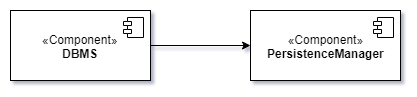
\includegraphics[scale=0.6]{implementation_and_testing/persistence.png}
	\end{center}
	\caption{I\&T - PersistenceManager}
\end{figure}

\subsubsection{AuthenticationManager}
Nearly every core-component require the \textit{AuthenticationManager} to work properly. It is to be integrated with the \textit{PersistenceManager}. A driver will simulate every possible authentication request.
\begin{figure}[H]
	\begin{center}
		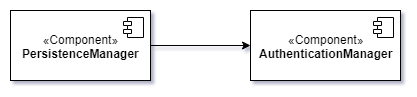
\includegraphics[scale=0.6]{implementation_and_testing/authentication.png}
	\end{center}
	\caption{I\&T - AuthenticationManager}
\end{figure}

\subsubsection{CalendarManager}
The \textit{CalendarManager}'s components interact all with \textit{AuthenticationManager} and \textit{PersistenceManager}, and so each component will be integrated with them. Since all \textit{CalendarManager}'s components offers an external interface to be exposed as RESTful services, a driver for each one of this components will be needed.\\
The \textit{CalendarManager}'s components are strictly correlated and so, in order to minimize the number of drivers and stubs, their integration order will be the following:\\
\indent 1. \textit{ScheduleManager} and \textit{PreferenceManager} are to be integrated with \textit{AuthenticationManager} and \textit{PersistenceManager}.
\begin{figure}[H]
	\begin{center}
		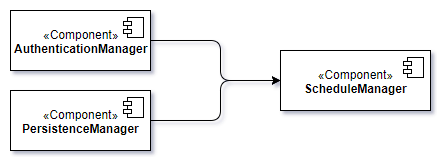
\includegraphics[scale=0.6]{implementation_and_testing/calendar_manager/schedule.png}
	\end{center}
	\caption{I\&T - ScheduleManager}
\end{figure}
\begin{figure}[H]
	\begin{center}
		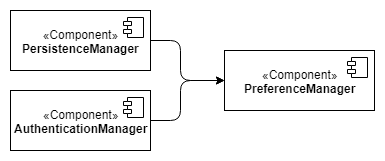
\includegraphics[scale=0.6]{implementation_and_testing/calendar_manager/preference.png}
	\end{center}
	\caption{I\&T - PreferenceManager}
\end{figure}

2. \textit{PathManager} is to be integrated with \textit{PersistenceManager}, \textit{AuthenticationManager}, \textit{GoogleMaps APIs}, \textit{PreferenceManager} and \textit{ScheduleManager}, following this order no stubs will be needed to perform the integration. It is required another driver, beside the one used to test the external interface, in order to simulate the calls performed by \textit{EventManager} to \textit{PathManager}.
\begin{figure}[H]
	\begin{center}
		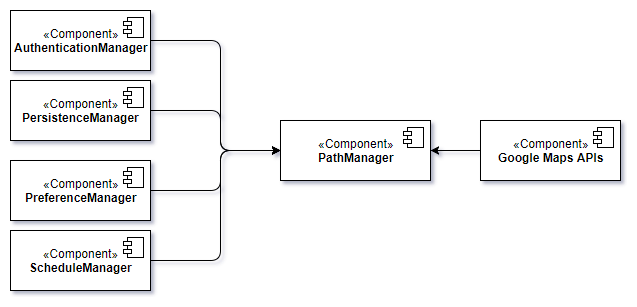
\includegraphics[scale=0.55]{implementation_and_testing/calendar_manager/path.png}
	\end{center}
	\caption{I\&T - PathManager}
\end{figure}

3. \textit{EventManager} is to be integrated with \textit{PersistenceManager}, \textit{AuthenticationManager}, \textit{ScheduleManager} and \textit{PathManager}, following this order no additional drivers or stubs will be needed.
\begin{figure}[H]
	\begin{center}
		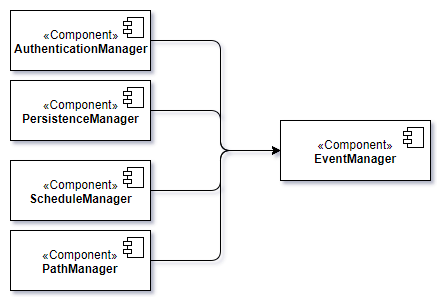
\includegraphics[scale=0.55]{implementation_and_testing/calendar_manager/event.png}
	\end{center}
	\caption{I\&T - EventManager}
\end{figure}

\subsubsection{TripManager}
\textit{TripManager} is to be integrated with \textit{PersistenceManager}, \textit{AuthenticationManager} and then with TSP APIs. Following this order a stub will be needed for the methods of \textit{TSP APIs} called by \textit{TripManager}. The driver needed for this module will simulate user's requests related to the trips-arranging methods provided.
\begin{figure}[H]
	\begin{center}
		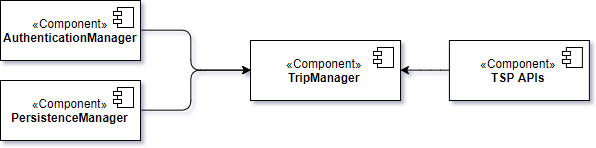
\includegraphics[scale=0.6]{implementation_and_testing/trip.png}
	\end{center}
	\caption{I\&T - TripManager}
\end{figure}

\subsubsection{NotificationManager}
\textit{NotificationManager} interacts only with \textit{GCM APIs} and so it is to be integrated with.
\begin{figure}[H]
	\begin{center}
		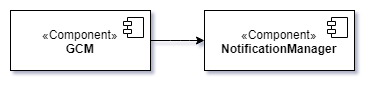
\includegraphics[scale=0.6]{implementation_and_testing/notification.png}
	\end{center}
	\caption{I\&T - NotificationManager}
\end{figure}

\subsubsection{ComplicationManager}
\textit{ComplicationManager} is to be integrated with \textit{PersistenceManager}, \textit{TSP APIs}, \textit{GoogleMaps APIs}, \textit{Weather API's} and \textit{NotificationManager}, following this order a stub will be needed for the methods of \textit{NotificationManager} called by \textit{ComplicationManager} ( basically when \textit{ComplicationManager} will have to notify the user's it will try to forward notification that will be received by the stub).
The integration of the three external APIs can be integrated in any possible order, since the interactions are independent from one another.
\begin{figure}[H]
	\begin{center}
		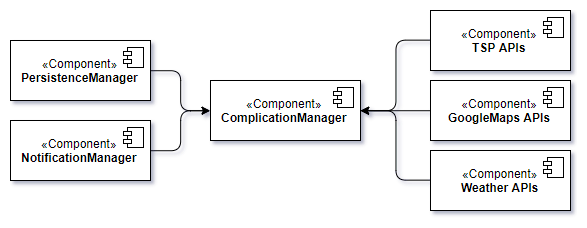
\includegraphics[scale=0.6]{implementation_and_testing/complication.png}
	\end{center}
	\caption{I\&T - ComplicationManager}
\end{figure}

\subsubsection{Overall integration of the Application Server}
The following picture is just a recap of the integration and test plan of the \textit{Application Server}. The integration order starts from the top of the picture and end in the bottom.
\begin{figure}[H]
	\begin{center}
		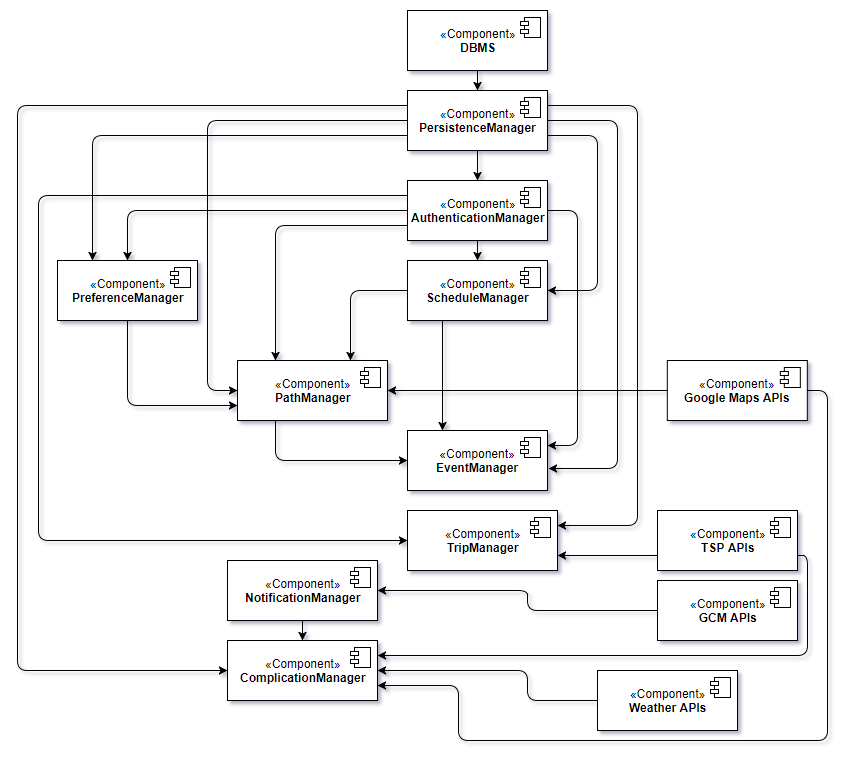
\includegraphics[scale=0.6]{implementation_and_testing/app_server_I&T.png}
	\end{center}
	\caption{I\&T - Application Server}
\end{figure}
\newpage
\subsubsection{WebServer}
In the web server subsystem the \textit{WebController} component is to be integrated with \textit{JavaServerPages} and then with \textit{Google Polylines APIs}. 
\begin{figure}[H]
	\begin{center}
		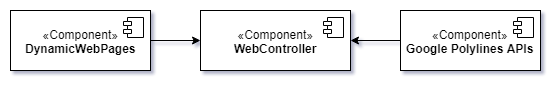
\includegraphics[scale=0.7]{implementation_and_testing/web.png}
	\end{center}
	\caption{I\&T - WebServer}
\end{figure}

\subsubsection{AppMobile}
The order of integration and testing of the \textit{AppMobile}'s components is the following: first \textit{DBManager} with \textit{LocalDBMS} and then \textit{ApplicationController} with \textit{DBManager}, \textit{GUIManager}, \textit{GCM API's} and \textit{Google Polylines APIs}. 
\begin{figure}[H]
	\begin{center}
		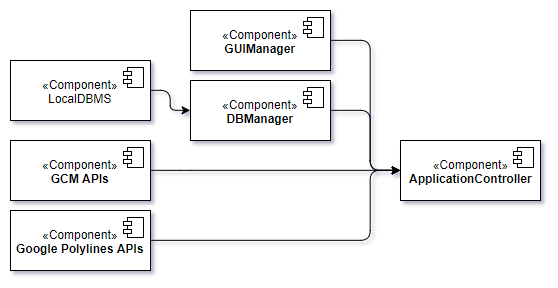
\includegraphics[scale=0.7]{implementation_and_testing/app.png}
	\end{center}
	\caption{I\&T - AppMobile}
\end{figure}
\newpage
\subsection{Subsystems integration Sequence}
Once all subsystem will be fully integrated this is the order in which they are to be integrated together in order to deploy the full Travlendar+ infrastructure.
\begin{figure}[H]
	\begin{center}
		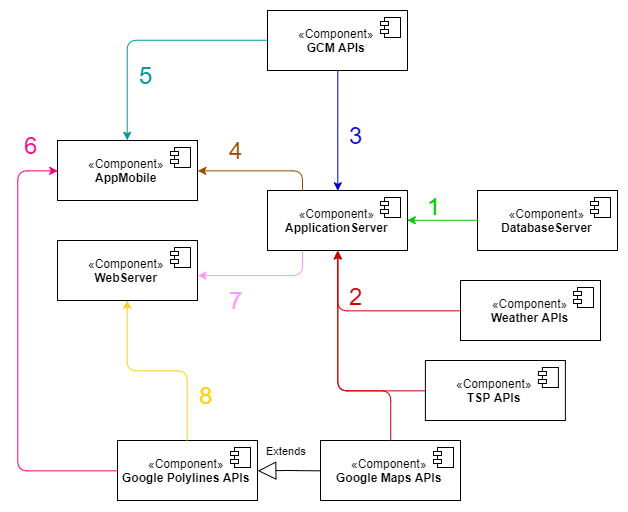
\includegraphics[scale=0.7]{implementation_and_testing/subsystem_integration.png}
	\end{center}
	\caption{I\&T - AppMobile}
\end{figure}